\documentclass[11pt]{article}
\usepackage[letterpaper,margin=1in]{geometry}
\usepackage{listings}
\usepackage{url}
\usepackage{hyperref}
\usepackage{textcomp}
\usepackage{graphicx}
\usepackage{underscore}
\lstset{%
  basicstyle=\small\ttfamily,
  mathescape=true,
  upquote=true,
}

\usepackage{amsmath,amsbsy,amsfonts,amssymb,amsthm,color,dsfont,mleftright,commath}

\def\ddefloop#1{\ifx\ddefloop#1\else\ddef{#1}\expandafter\ddefloop\fi}

% \bbA, \bbB, ...
\def\ddef#1{\expandafter\def\csname bb#1\endcsname{\ensuremath{\mathbb{#1}}}}
\ddefloop ABCDEFGHIJKLMNOPQRSTUVWXYZ\ddefloop

% \cA, \cB, ...
\def\ddef#1{\expandafter\def\csname c#1\endcsname{\ensuremath{\mathcal{#1}}}}
\ddefloop ABCDEFGHIJKLMNOPQRSTUVWXYZ\ddefloop

% \vA, \vB, ..., \va, \vb, ...
\def\ddef#1{\expandafter\def\csname v#1\endcsname{\ensuremath{\boldsymbol{#1}}}}
\ddefloop ABCDEFGHIJKLMNOPQRSTUVWXYZabcdefghijklmnopqrstuvwxyz\ddefloop

% \valpha, \vbeta, ...,  \vGamma, \vDelta, ...,
\def\ddef#1{\expandafter\def\csname v#1\endcsname{\ensuremath{\boldsymbol{\csname #1\endcsname}}}}
\ddefloop {alpha}{beta}{gamma}{delta}{epsilon}{varepsilon}{zeta}{eta}{theta}{vartheta}{iota}{kappa}{lambda}{mu}{nu}{xi}{pi}{varpi}{rho}{varrho}{sigma}{varsigma}{tau}{upsilon}{phi}{varphi}{chi}{psi}{omega}{Gamma}{Delta}{Theta}{Lambda}{Xi}{Pi}{Sigma}{varSigma}{Upsilon}{Phi}{Psi}{Omega}{ell}\ddefloop

\newcommand\braces[1]{\{#1\}}

\theoremstyle{definition}
\newtheorem{problem}{Problem}
\newenvironment{solution}{\noindent\emph{Solution.}}{\hfill$\square$}

%-------------------------------------------------------------------------------

\title{COMS 4771 Fall 2016 Homework 1 \\ Due Wednesday, September 21}
\author{Jin Tack Lim, jl4312
  }
\date{%
  }

\begin{document}
\maketitle

\newpage

%-------------------------------------------------------------------------------

\begin{problem}[Nearest neighbors; 20 points]
  \label{prob:nn}
  Download the OCR image data set \texttt{ocr.mat} from Courseworks,

  and load it into MATLAB:
  \lstset{language=Matlab}
  \begin{lstlisting}
    load('ocr.mat')
  \end{lstlisting}
  Or Python:
  \lstset{language=Python}
  \begin{lstlisting}
    from scipy.io import loadmat
    ocr = loadmat('ocr.mat')
  \end{lstlisting}

  The unlabeled training data (i.e., feature vectors) are contained in
  a matrix called \texttt{data} (one point per row), and the
  corresponding labels are in a vector called \texttt{labels}.
  The test feature vectors and labels are in, respectively,
  \texttt{testdata} and \texttt{testlabels}.
  In MATLAB, you can view an image (say, the first one) in the
  training data with the following commands:
  \lstset{language=Matlab}
  \begin{lstlisting}
    imagesc(reshape(data(1,:),28,28)');
  \end{lstlisting}
  If the colors are too jarring for you, try the following:
  \begin{lstlisting}
    colormap(1-gray);
  \end{lstlisting}
  In Python, to view the first image, try the following (ideally, from
  IPython or Jupyter Notebook):
  \lstset{language=Python}
  \begin{lstlisting}
    import matplotlib.pyplot as plt
    from matplotlib import cm
    plt.imshow(ocr['data'][0].reshape((28,28)), cmap=cm.gray_r)
    plt.show()
  \end{lstlisting}

  Write a function that implements the $1$-nearest neighbor classifier
  with Euclidean distance.
  Your function should take as input a matrix of training feature
  vectors \texttt{X} and a vector of the corresponding labels
  \texttt{Y}, as well as a matrix of test feature vectors
  \texttt{test}.
  The output should be a vector of predicted labels \texttt{preds} for
  all the test points.
  Naturally, you should not use (or look at the source code for) any library
  functions for computing pairwise distsances or nearest neighbor queries.
  If in doubt about what is okay to use, just ask.
  Note that for efficiency, you should use matrix/vector operations (rather
  than, say, a bunch of for-loops).\footnote{%
    \url{http://www.mathworks.com/help/matlab/matlab_prog/vectorization.html}%
  }

  Instead of using your 1-NN code directly with \texttt{data} and
  \texttt{labels} as the training data, do the following.
  For each value $n \in \braces{1000,2000,4000,8000}$,
  \begin{itemize}
    \item
      Draw $n$ random points from \texttt{data}, together with their
      corresponding labels.
      In MATLAB, use \lstinline{sel = randsample(60000,$n$)} to pick the
      $n$ random indices, and \texttt{data(sel,:)} and
      \lstinline{labels(sel)} to select the examples; in Python, use
      \lstinline{sel = random.sample(xrange(60000),$n$)} (after
      \lstinline{import random}),
      \lstinline{ocr['data'][sel].astype('float')}, and
      \lstinline{ocr['labels'][sel]}.

    \item
      Use these $n$ points as the training data and \texttt{testdata}
      as the test points, and compute the test error rate of the
      $1$-NN classifier.

  \end{itemize}
  A plot of the error rate (on the y-axis) as a function of $n$ (on
  the x-axis) is called a \emph{learning curve}.
  We get an estimate of this curve by using the test error rate in
  place of the (true) error rate.

  Repeat the (random) process described above ten times, independently.
  Produce an estimate of the learning curve plot using the average of
  these test error rates (that is, averaging over ten repetitions).
  Add error bars to your plot that extend to one standard deviation
  above and below the means.
  Ensure the plot axes are properly labeled.

  What to submit:
  (1) learning curve plot, (2) source code (in a separate file).
\end{problem}

\begin{solution}

1. Figure~\ref{fig:lc} shows the learning curve plot~\cite{gnuplot-so} with 1000, 2000, 4000 and 8000 training data set. Table~\ref{tbl:lc} shows the raw data.

2. knn-rand.py

\begin {figure}[h]
    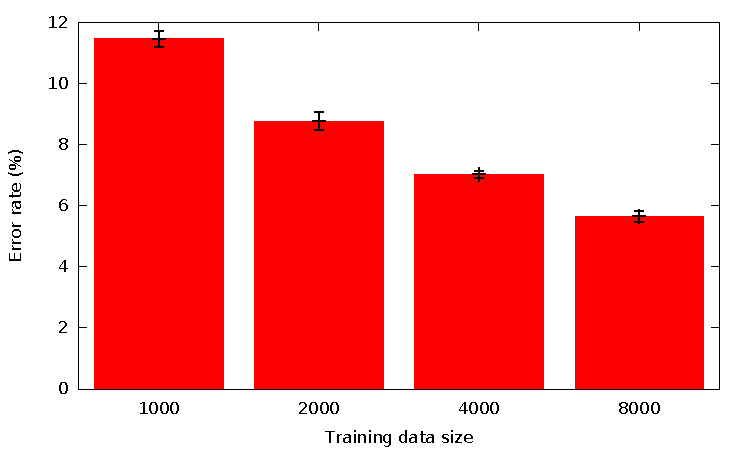
\includegraphics{figures/fig1}
	\caption{Learning curve}
	\label{fig:lc}
\end {figure}

\begin{table}[h]
\centering
\begin{tabular}{|c|r|r|}
\hline
\textbf{training size} & \multicolumn{1}{c|}{\textbf{error rate (\%)}} & \multicolumn{1}{c|}{\textbf{stdev}} \\ \hline
1000                   & 11.454                                        & 0.265                               \\ \hline
2000                   & 8.765                                         & 0.299                               \\ \hline
4000                   & 7.026                                         & 0.125                               \\ \hline
8000                   & 5.655                                         & 0.183                               \\ \hline
\end{tabular}
\caption{Learning curve data}
\label{tbl:lc}
\end{table}

\end{solution}

\newpage

%-------------------------------------------------------------------------------

\begin{problem}[Prototype selection; 20 points]
  Prototype selection is a method for speeding-up nearest neighbor search that
  replaces the training data with a smaller subset of \emph{prototypes} (which
  could be data points themselves).
  For simplicity, assume that 1-NN is used with Euclidean distance.
  So a prototype selection method simply takes as input:
  \begin{itemize}
    \item
      the training data $\{ (\vx_i,y_i) \}_{i=1}^n$ from $\bbR^d \times
      \{0,1,\dotsc,9\}$ (say), and

    \item
      a positive integer $m$;

  \end{itemize}
  it should return $m$ labeled pairs $\{(\tilde\vx_i,\tilde y_i)\}_{i=1}^m$,
  each from $\bbR^d \times \{0,1,\dotsc,9\}$.

  Design a method for choosing prototypes, where the goal is for the 1-NN
  classifier based on the prototypes to have good test accuracy.
  Implement your algorithm; use it to select prototypes for the OCR data
  set, and evaluate the test error rate of the 1-NN classifier based on the
  selected prototypes.
  You should use the whole training data set as input (i.e., all $n=60000$ data
  points), but vary the number of selected prototypes $m$ in the set $\{ 1000,
  2000, 4000, 8000 \}$.
  If your procedure is randomized, repeat it at least ten times (for each $m$)
  to properly assess its performance.

  What to submit:
  \begin{enumerate}
    \item
      A brief description of your method (in words).

    \item
      Concise and unambiguous pseudocode for your algorithm.

    \item
      A table of the test error rates for the different values of $m$ you try.
      (Report averages and standard deviations if your procedure is randomized.)

    \item
      Source code (in a separate file).

  \end{enumerate}

\end{problem}

\begin{solution}

1. There are two observations.

 1) The err rate for each label is different.
For example, error rate for label 1 is pretty low compared to others probably due to a simple shape of letter 1.


 2) As we can see from the result of problem 1, the more training set is given, the accuracy gets better.

Based on those observations, my method is to sample different number of points for each label depending on error rates of the label respectively. In other words, sample small number of points for a label with low error rate, and sample large number of points for a label with high error rate. 
The rationale behind the idea is that sampling small number of points for a low-error-rate label does not increase error rate much due to a simple shape (i.e. not much variation). On the other hand, sampling a large number of points for a high-error-rate label will decrease an error rate much based on the observation with different training size in problem1.

2.
\begin{verbatim}
prototype_data prototype_select(training_data, training_label, prototype_size)
{
    p_data[0:9] = partition training_data based on its label(0~9)
	
    // sample size is predefined by looking at error rate of each labels
    // and doing trial-and-error to find reasonable accurate increasement
    // I used [4, 1.5, 11.5, 13, 14, 10, 4, 10, 20, 12] * prototype_size/100
    sample_size[0:9] = [s0, s1, … , s9] where sum(s0:s9) = prototype_size
	
    for i in 0 to 9
        prototype_data += sample(p_data[i], sample_size[i])
	
    return prototype_data
}
\end{verbatim}

3.
\begin{table}[h]
\centering
\begin{tabular}{|c|r|r|r|}
\hline
\textbf{training size} & \multicolumn{1}{c|}{\textbf{error rate (\%)}} & \multicolumn{1}{l|}{\textbf{\begin{tabular}[c]{@{}l@{}}accuracy\\ improvement (\%)\end{tabular}}} & \multicolumn{1}{c|}{\textbf{stdev}} \\ \hline
1000                   & 10.934                                        & 4.54                                                                                              & 0.415                               \\ \hline
2000                   & 8.001                                         & 8.72                                                                                              & 0.236                               \\ \hline
4000                   & 6.169                                         & 12.20                                                                                             & 0.236                               \\ \hline
8000                   & 4.937                                         & 12.70                                                                                             & 0.127                               \\ \hline
\end{tabular}
\caption{Test error rates}
\end{table}

4. knn-proto.py
\end{solution}

\newpage

%-------------------------------------------------------------------------------

\begin{problem}[Probability; 10 points]
  Suppose you have an urn containing $100$ colored balls.
  Each ball is painted with one of five possible colors from the color
  set $\cC := \braces{ \text{red}, \text{orange}, \text{yellow},
  \text{green}, \text{blue} }$.
  For each $c \in \cC$, let $n_c$ denote the number of balls in the
  urn with color $c$.
  \begin{enumerate}
    \item[(a)]
      Suppose you pick two balls uniformly at random \emph{with replacement}
      from the urn.
      What is the probability that they have different colors?
      Briefly explain your answer.

    \item[(b)]
      Suppose you want to maximize the probability from part (a).
      You are allowed to paint all of the balls in the urn, each with any color
      from $\cC$.
      How many balls in the urn would you paint with each color in $\cC$?
      Briefly explain your answer.

  \end{enumerate}

\end{problem}

\begin{solution}

(a) $1 - (1/n_{red})^2 - (1/n_{orange})^2 - (1/n_{yellow})^2 - (1/n_{green})^2 - (1/n_{blue})^2$

The probability that two balls have different colors is a complementary set of the probability that two balls have the same color.


(b) 20 balls for each color

Intuitively, when the colors of balls are evenly distributed, the probability that two balls have different colors is maximized.

To prove it formally, we can start from the simplied case: there are 40 balls
and two colors. Then compare the probability when painting 20 balls for each
color and all other cases.

When painting 20 balls for each, the probability is $1 - (1/20)^2 - (1/20)^2$

All other cases can be represented by painting (20-k) in one color and (20+k)
in the other color where $0<k<20$. The probability is $1 - (1/(20-k))^2 -
(1/(20+k))^2$

By doing subtraction, we can easily prove that the former is always greater
than the latter with any $k$ value in the range. We can also easily extend this 
to cases with more than two colors.

\end{solution}

\bibliographystyle{plain}
\bibliography{references}
\end{document}

